\documentclass{article}
\usepackage{graphicx} % Required for inserting images
\usepackage{amsmath}
\usepackage{tikz}
\usepackage{listings}
\usepackage{xcolor}

\title{A Derivation for the Backup Camera Trajectory Calculation}
\author{Chase Mayer}
\date{July 2026}

\begin{document}

\newcommand{\dxdt}{\frac{\mathrm{d}x}{\mathrm{d}t}}
\newcommand{\dydt}{\frac{\mathrm{d}y}{\mathrm{d}t}}

% Configure listings style
\lstdefinestyle{mystyle}{
    basicstyle=\ttfamily\footnotesize,
    breaklines=true,
    numbers=left,
    numbersep=5pt,
    tabsize=2
}
\lstset{style=mystyle}

\maketitle

\section{Introduction}

The backup camera overlay needs to know all the details of the SEV's trajectory to provide an accurate guide for the driver. In this document, we detail the derivation of the formula for calculating that trajectory.

From the SEV we receive the orientations of all 6 wheel modules. Each of these modules gives us an associated equation constraining the SEV's movement. To solve for the SEV's total movement (x-movement $\dxdt$, y-movement $\dydt$, and yaw rate $\frac{\mathrm{d}\theta}{\mathrm{d}t}=\omega$), we need to solve -- or approximate -- the system of equations.

\section{Derivation}
\subsection{Setup}

First, we define our coordinate system. The center of the SEV wheelbase is the origin, with the positive x-direction pointing to the side and the positive y-direction pointing to the front.

Let $W$ be the width of the wheelbase (from wheel center to wheel center). Let $L$ be the wheelbase length. The positions of all the wheels are shown in Figure~\ref{fig:robot_geometry}.

\begin{figure}[ht]
\centering
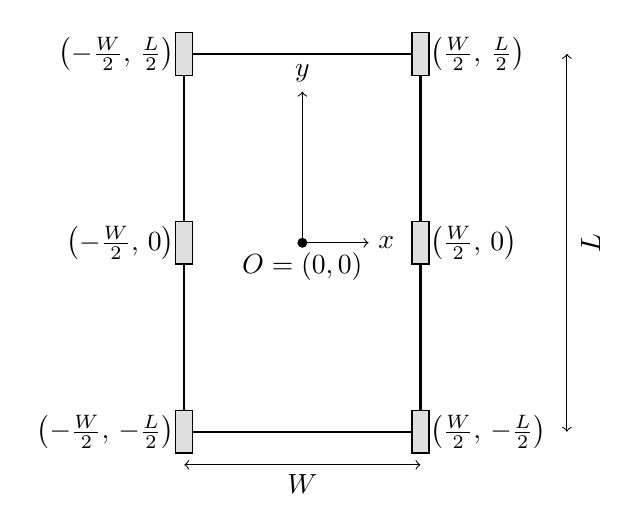
\begin{tikzpicture}[scale=1.2]

% Parameters for drawing only
\def\W{2.5}
\def\L{4.0}
\def\wheelw{0.18}
\def\wheelh{0.45}

% Box
\draw[thick] (-\W/2,-\L/2) rectangle (\W/2,\L/2);

% Coordinate axes
\draw[->] (0,0) -- (0.7,0) node[right] {$x$};
\draw[->] (0,0) -- (0,1.6) node[above] {$y$};

% Origin
\fill (0,0) circle (1.5pt);
\node[below] at (0,0) {$O=(0,0)$};

% Front left wheel
\draw[fill=gray!25]
(-\W/2-\wheelw/2,\L/2-\wheelh/2)
rectangle
(-\W/2+\wheelw/2,\L/2+\wheelh/2);
\node[left] at (-\W/2,\L/2)
{$\left(-\frac{W}{2},\,\frac{L}{2}\right)$};

% Front right wheel
\draw[fill=gray!25]
(\W/2-\wheelw/2,\L/2-\wheelh/2)
rectangle
(\W/2+\wheelw/2,\L/2+\wheelh/2);
\node[right] at (\W/2,\L/2)
{$\left(\frac{W}{2},\,\frac{L}{2}\right)$};

% Middle left wheel
\draw[fill=gray!25]
(-\W/2-\wheelw/2,-\wheelh/2)
rectangle
(-\W/2+\wheelw/2,\wheelh/2);
\node[left] at (-\W/2,0)
{$\left(-\frac{W}{2},\,0\right)$};

% Middle right wheel
\draw[fill=gray!25]
(\W/2-\wheelw/2,-\wheelh/2)
rectangle
(\W/2+\wheelw/2,\wheelh/2);
\node[right] at (\W/2,0)
{$\left(\frac{W}{2},\,0\right)$};

% Rear left wheel
\draw[fill=gray!25]
(-\W/2-\wheelw/2,-\L/2-\wheelh/2)
rectangle
(-\W/2+\wheelw/2,-\L/2+\wheelh/2);
\node[left] at (-\W/2,-\L/2)
{$\left(-\frac{W}{2},\,-\frac{L}{2}\right)$};

% Rear right wheel
\draw[fill=gray!25]
(\W/2-\wheelw/2,-\L/2-\wheelh/2)
rectangle
(\W/2+\wheelw/2,-\L/2+\wheelh/2);
\node[right] at (\W/2,-\L/2)
{$\left(\frac{W}{2},\,-\frac{L}{2}\right)$};

% Dimension labels
\draw[<->] (-\W/2,-2.35) -- (\W/2,-2.35);
\node at (0,-2.55) {$W$};

\draw[<->] (2.8,-\L/2) -- (2.8,\L/2);
\node[rotate=90] at (3.05,0) {$L$};

\end{tikzpicture}
\caption{Top-down view of the six-wheel SEV. The origin is at the geometric center of the chassis, with wheel locations expressed symbolically in terms of chassis width $W$ and length $L$.}
\label{fig:robot_geometry}
\end{figure}

Consider a point $P$ on the SEV wheelbase. We begin our derivation by solving for $\vec{v_P}$, the instantaneous velocity at $P$. We are given the linear velocity of the SEV $\vec{v}=\langle \dxdt, \dydt \rangle$ and the rotational velocity $\omega$. We know that $\vec{v_P}$ is the sum of $\vec{v}$ and some vector $\vec{v_{rot}}$, the velocity due to rotation:
\begin{equation*}
    \vec{v_P}=\vec{v}+\vec{v_{rot}}
\end{equation*}
The direction of $\vec{v_{rot}}$ will be perpendicular to $\vec{P}$, and its magnitude will be proportional to $\omega$:
\begin{equation*}
    \vec{v_{rot}}=\omega \langle -P_y, P_x \rangle
\end{equation*}
And thus,
\begin{equation}
\label{eq:vel_at_point}
    \vec{v_P} = \vec{v} + \omega \langle -P_y, P_x \rangle
\end{equation}
Given this equation and the velocity at each wheel (i.e. $\vec{v_P}$ for point $P$ located on a wheel), we can solve for $\vec{v}$ and $\omega$.

\subsection{Solution Using Wheel Orientations}
From the SEV, we obtain data about the orientation of each wheel. If we knew the instantaneous speed at each wheel, we could directly insert it into Equation~\ref{eq:vel_at_point}. However, directly using the speed of each wheel would be unreliable when the vehicle is parked. Simply using the orientation of each wheel, denoted by the unit vector $\hat{s}$, provides more than enough information, with no need for speed data. We can then define a vector $\vec{n}$ that is perpendicular to the wheel direction, as shown in Figure~\ref{fig:wheel_vectors}.
\begin{equation*}
    \vec{n} = \langle -s_y, s_x \rangle
\end{equation*}

\begin{figure}[ht]
\centering
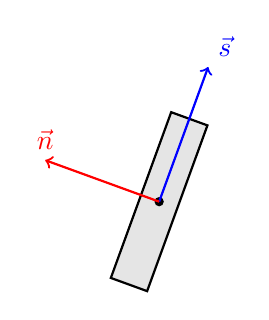
\begin{tikzpicture}[scale=1.4]

% Wheel orientation (degrees)
\def\theta{20}

% Wheel dimensions
\def\wheelW{0.35}
\def\wheelL{1.6}

% Draw wheel
\begin{scope}[rotate=-\theta]
    \draw[fill=gray!20, thick]
        (-\wheelW/2,-\wheelL/2)
        rectangle
        (\wheelW/2,\wheelL/2);
\end{scope}

% Wheel center
\fill (0,0) circle (1.2pt);

% Rolling direction vector S
\draw[->, thick, blue]
    (0,0) -- ({1.3*sin(\theta)},{1.3*cos(\theta)})
    node[above right] {$\vec{s}$};

% Normal vector N
\draw[->, thick, red]
    (0,0) -- ({-1.1*cos(\theta)},{1.1*sin(\theta)})
    node[above] {$\vec{n}$};

\end{tikzpicture}
\caption{Top-down view of a wheel showing its rolling direction $\vec{s}$ and lateral normal direction $\vec{n}$.}
\label{fig:wheel_vectors}
\end{figure}

The normal vector $\vec{n}$ is perpendicular to the instantaneous velocity at the wheel, $\vec{v_P}$. We thus obtain the following speed-independent relation:
\begin{equation}
\label{eq:normal}
    \vec{n} \cdot \vec{v_P} = 0
\end{equation}

Substituting our expression for $\vec{v_P}$ from Equation~\ref{eq:vel_at_point}:
\begin{align*}
    \vec{n} \cdot (\vec{v} + \omega \langle -P_y, P_x \rangle) &= 0 \\
    n_x(v_x - \omega P_y) + n_y(v_y + \omega P_x) &= 0 \\
    n_x v_x + n_y v_y + (-n_x P_y + n_y P_x)\omega &= 0 \\
    -s_y v_x + s_x v_y + (s_x P_x + s_y P_y)\omega &= 0
\end{align*}

We obtain an equation of this form for each of the six wheels, each with their unique coordinates $P$. Writing the resulting system of equations in matrix form:

\begin{equation}
\label{eq:system_of_wheels}
    \begin{bmatrix}
        -s_y & s_x & s_x x_0+s_y y_0 \\
        -s_y & s_x & s_x x_1+s_y y_1 \\
        -s_y & s_x & s_x x_2+s_y y_2 \\
        -s_y & s_x & s_x x_3+s_y y_3 \\
        -s_y & s_x & s_x x_4+s_y y_4 \\
        -s_y & s_x & s_x x_5+s_y y_5
    \end{bmatrix}
    \begin{bmatrix}
        v_x \\
        v_y \\
        \omega
    \end{bmatrix}
    =
    \mathbf{0}
\end{equation}
where $(x_n, y_n)$ is the location of the $n\text{th}$ wheel in the coordinate system outlined in Figure~\ref{fig:robot_geometry}. We refer to the first matrix hereafter as the \emph{wheel matrix}.

\subsection{Solving the System of Equations}

If a vector can be multiplied with a given matrix, such as our wheel matrix above, and produce the zero vector as a result, that vector is said to lie in the matrix's \emph{null space}. Thus, all solutions to the above system of equations lie in the wheel matrix's null space.

The vector $\langle 0, 0, 0 \rangle$ will always lie in the null space of the wheel matrix. Since the system of equations is overdetermined (there are more equations than unknowns), $\mathbf{0}$ is likely to be the only solution to the system. Solving the above system directly will yield a result of $\dxdt=\dydt=\omega=0$. That is to say, the system will predict no motion whatsoever of the SEV. Though this "no-motion" solution does technically fulfill the constraints imposed by each wheel, it is obviously not helpful in predicting the SEV's trajectory.

Since we consider only the wheel orientations and not the wheel speeds, all vectors $\langle v_x, v_y, \omega \rangle = \lambda \hat{u}$ -- where $\hat{u}$ is the normalized trajectory of the SEV -- are valid solutions. Solving directly would yield the trivial solution where $\lambda = 0$. All of these solutions lie in the null space, though, and they are all scalar multiples of each other. Our goal, then, is to find the \emph{direction} of the null space. That is to say, we wish to find the shared direction of every vector in the null space. The null space direction is calculated in Python using numpy in Listing~\ref{lst:null_space}.

\begin{lstlisting}[language=Python, caption={Calculating the direction of the null space using numpy. Note that if the direction is too small, we understand the null space to contain only $\langle 0, 0, 0 \rangle$.}, label={lst:null_space}]
_, _, vt = np.linalg.svd(A)
motion_dir = vt[-1, :]

norm = np.linalg.norm(motion_dir)
if norm < 1e-9:
    dx_dt, dy_dt, dtheta_dt = 0.0, 0.0, 0.0
else:
    motion_dir = motion_dir / norm

    # Keep direction sign consistent frame-to-frame to avoid flickering.
    if prev_motion_dir is not None and np.dot(motion_dir, prev_motion_dir) < 0:
        motion_dir = -motion_dir

    prev_motion_dir = motion_dir.copy()
    dx_dt = float(MOTION_SCALE * motion_dir[0])
    dy_dt = float(MOTION_SCALE * motion_dir[1])
    dtheta_dt = float(MOTION_SCALE * motion_dir[2])
\end{lstlisting}

The definition of SVD and the reason it provides the direction of the null space is linear algebra outside the scope of this derivation. The null space direction, though, is used directly as the SEV trajectory, thus concluding this derivation.

\end{document}
